\subsection{Database Design}
Databasen bestod i første iteration af individuelle TXT filer som blev brugt som CSV filer. Dette lod os dele dataen op i de forskellige typer af objekter vi gerne ville have opbevaret, f.eks. Episode, Person og Movie, så hver type fik sin egen fil. På den måde undgik vi at indlæse alt vores data når vi skulle have fat i noget specifikt, og dermed spare ressourcer i form af tid og lagring.

\begin{comment}


\begin{figure}[H]
    \centering
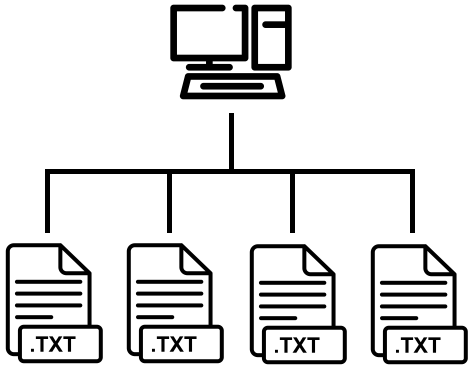
\includegraphics[scale = 0.35]{images/computer_to_txt_file_icon.png}
\caption{Database i form af tekst filer}
\end{figure}

\end{comment}

I anden iteration er der gjort brug af en SQL relationel database, på baggrund af kravene til anden iteration. Ud fra de objekter der findes i systemet har gruppen udarbejdet et UML diagram over databasedesignet, på en sådan måde at det som minimum opfylder 3. normalform. 
UML diagrammet over databasedesignet giver et godt overblik, og viser relationerne mellem de forskellige tabeller, ved crows foot notation. I figur \ref{fig:databaseUML} ses alle tabeller der eksistere i databasen. Her ses det at en "credit" kan have én "person", men at én "person" kan have én eller mange "jobs". 
\begin{figure}[H]
    \centering
    \makebox[\textwidth][c]{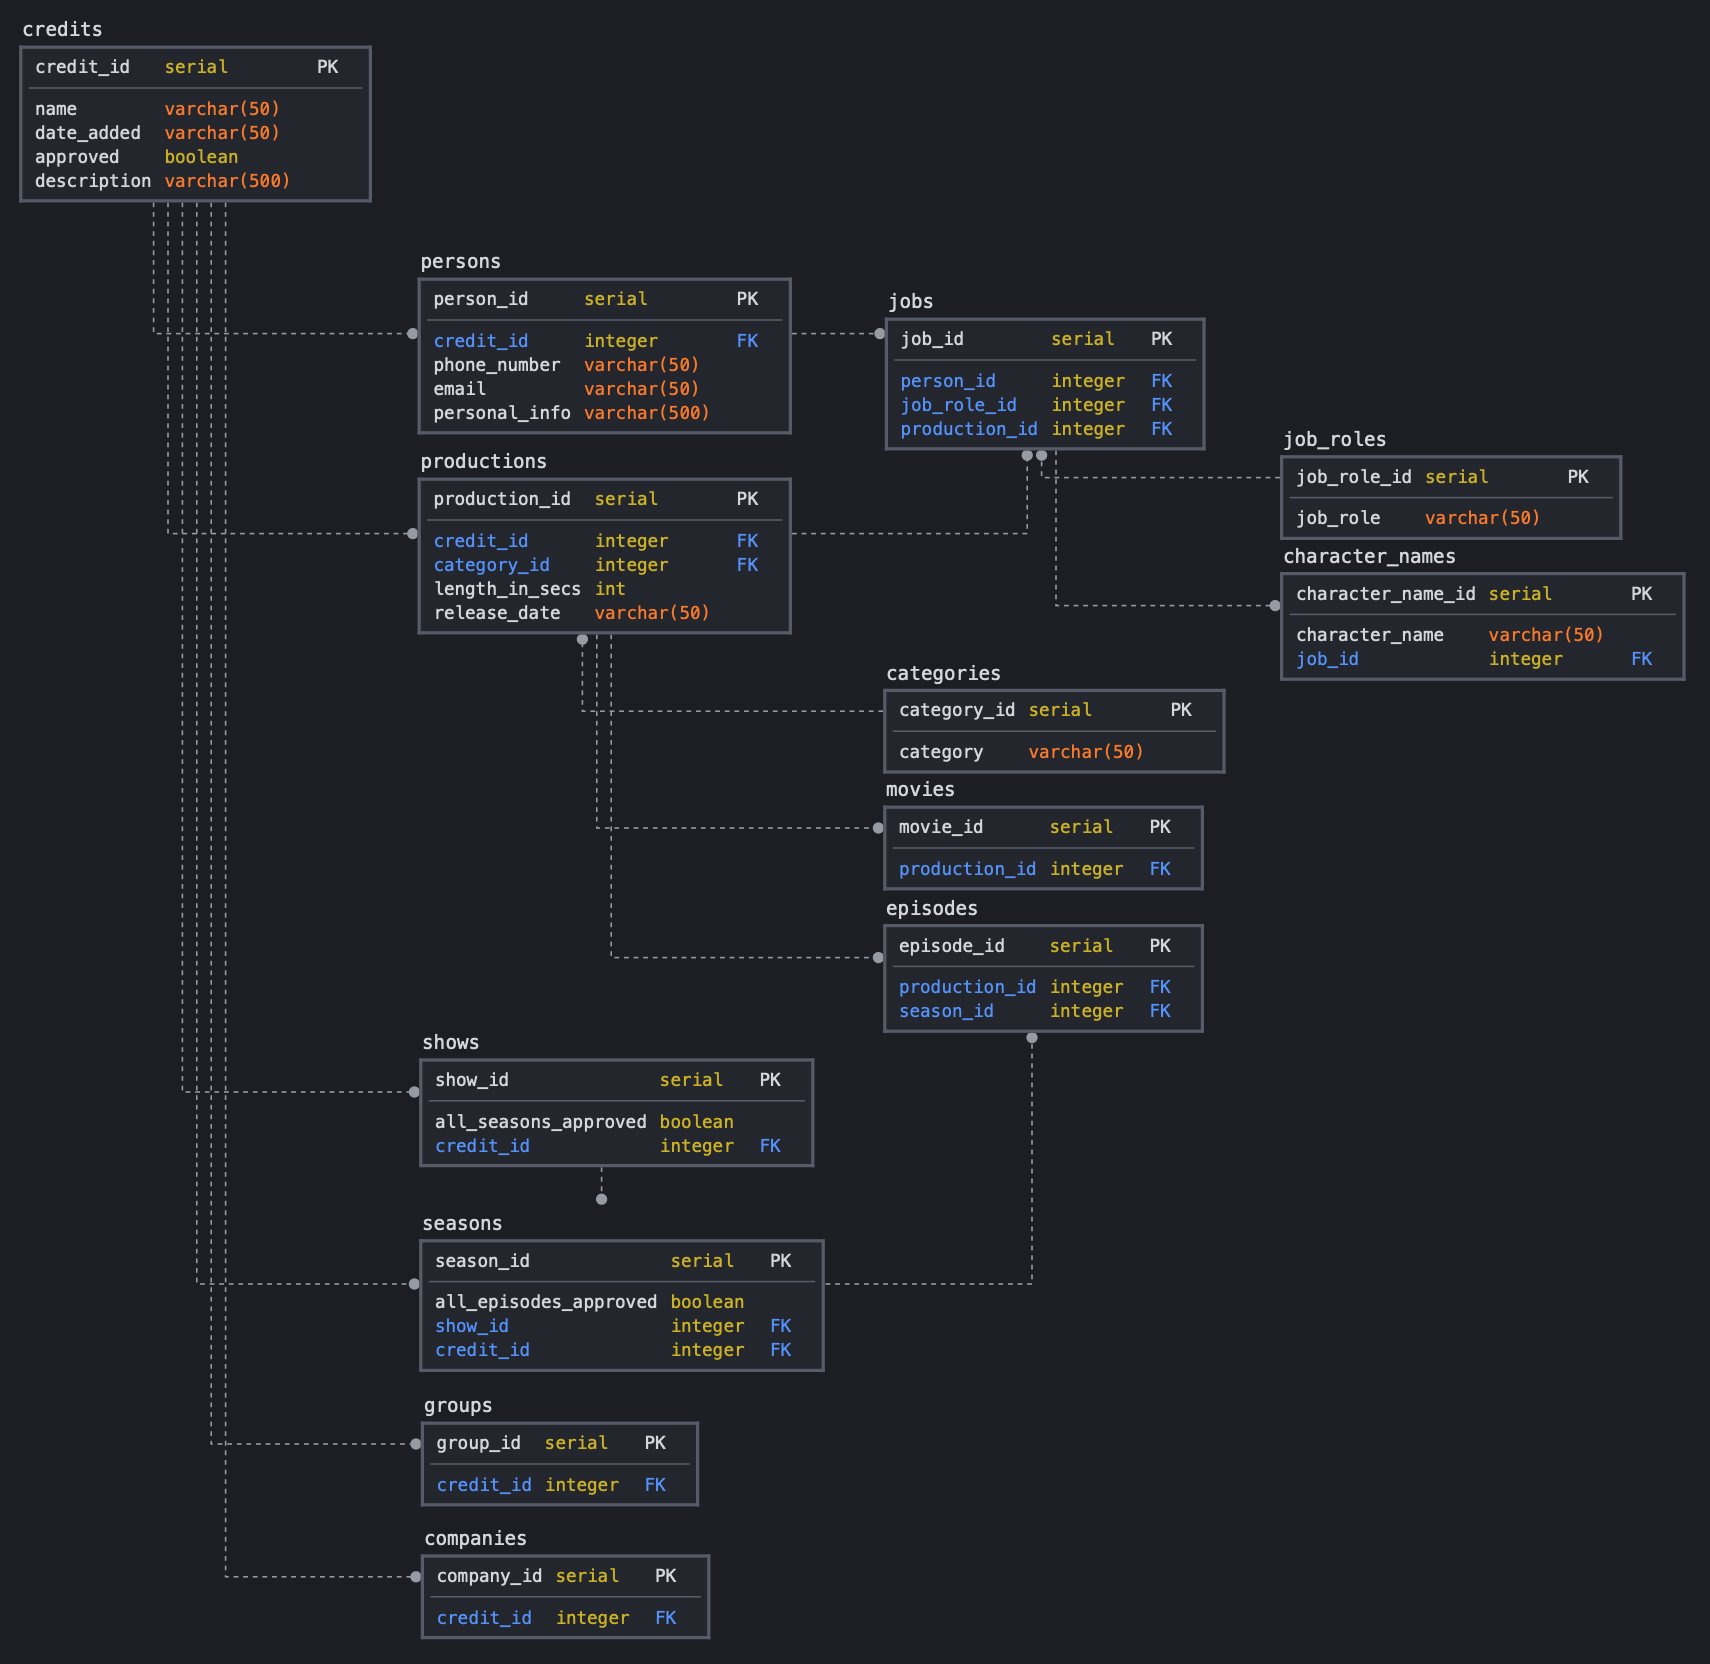
\includegraphics[width=1.25\textwidth]{images/Database design.png}}
    \caption{UML diagram over databasen}
    \label{fig:databaseUML}
\end{figure}